\renewcommand{\myname}{Md Kamruzzaman Kamrul (mkamrul@purdue.edu)}

\renewcommand{\report}{

\section*{Assignment Scope and Experimental Protocol}
\label{sec:scope}
This submission follows the assignment requirements in \texttt{Assignment Description/CS59300\_CVD\_HW2.pdf} and keeps the professor-provided starter-code entry points:
\begin{itemize}
\item Part 1: \texttt{main\_p1.py} (learnable alignment)
\item Part 2: \texttt{main\_p2.py} (scale-space blob detection)
\end{itemize}

All numbers below were re-generated from the current code and recorded in \texttt{logs/}. The report uses:
\begin{itemize}
\item \texttt{part1\_alignment\_runs.csv}, \texttt{part1\_quality\_metrics.csv/json}, \texttt{part1\_debug\_*.json}
\item \texttt{part2\_blob\_runs.csv}
\item \texttt{part2\_profile\_proxy\_per\_image.csv}, \texttt{part2\_profile\_proxy\_overall.csv}
\item \texttt{part2\_profile\_proxy\_eval.md/json}
\end{itemize}

\section*{Part 1: Learnable Alignment}
\label{sec:part1}

\subsection*{Mathematical Formulation and Notation}
\label{sec:p1-opt}
For a fixed reference channel $G$ and moving channel $C\in\{B,R\}$, I optimize 2D translation $(\theta_x,\theta_y)$:
\begin{equation}
\label{eq:p1-objective}
(\theta_x^\star,\theta_y^\star)=\arg\min_{\theta_x,\theta_y}\;\mathcal{L}\!\left(G,\mathcal{W}(C;\theta_x,\theta_y)\right),
\end{equation}
where $\mathcal{W}(\cdot)$ is differentiable warping implemented via \texttt{affine\_grid} and \texttt{grid\_sample}. The affine matrix is
\begin{equation}
\label{eq:p1-affine}
\mathbf{A}=\begin{bmatrix}
1&0&\theta_x\\
0&1&\theta_y
\end{bmatrix}.
\end{equation}
The gradient descent update is
\begin{equation}
\label{eq:p1-gd}
\theta^{(t+1)}=\theta^{(t)}-\eta\nabla_{\theta}\mathcal{L}\!\left(G,\mathcal{W}(C;\theta^{(t)})\right).
\end{equation}
I report results with two losses required by the assignment: NCC and MSE.

\subsection*{General Algorithmic Overview and Stages}
\label{sec:p1-overview}
I use a coarse-to-fine, restart-aware alignment pipeline:
\begin{enumerate}
\item \textbf{Preprocess and channel split}: read stacked grayscale plate, divide into $B,G,R$, crop borders.
\item \textbf{Construct stage-wise image representations}: for each scale $\{0.25,0.5,1.0\}$ I downsample and compute both intensity and Sobel-edge maps.
\item \textbf{Stage optimization}: optimize translations first in edge space, then in intensity space.
\item \textbf{Progressive refinement}: initialize each finer stage with the best shift from the previous stage.
\item \textbf{Final composition}: warp $B$ and $R$ to $G$ and stack RGB.
\end{enumerate}

How the image representation changes by stage:
\begin{itemize}
\item Stage 1 (0.25): broad global structure dominates; helps avoid bad local minima.
\item Stage 2 (0.50): restores medium-frequency structures; improves shift precision.
\item Stage 3 (1.00): fine alignment at full resolution; resolves residual fringes.
\end{itemize}

\subsection*{Implementation Choices, Runtime, and Step Statistics}
\label{sec:p1-impl}
Fixed hyperparameters:
\begin{itemize}
\item Scale 0.25: lr=0.02, 500 max steps, 3 restarts.
\item Scale 0.50: lr=0.01, 700 max steps.
\item Scale 1.00: lr=0.004, 1200 max steps.
\item Early-stop patience after edge phase (to reduce unnecessary iterations).
\end{itemize}

\begin{table}[htbp]
\centering
\small
\begin{tabular}{c|cc|cc}
\hline
Image & NCC runtime (s) & MSE runtime (s) & NCC total steps (B+R) & MSE total steps (B+R)\\
\hline
1 & 6.2983 & 5.5330 & 3211 & 3375\\
2 & 6.4114 & 5.9746 & 3349 & 3419\\
3 & 5.4504 & 6.1206 & 2826 & 3542\\
4 & 6.0420 & 6.5746 & 3107 & 3615\\
5 & 6.5002 & 6.0591 & 3220 & 3444\\
6 & 4.3645 & 6.9257 & 2246 & 3423\\
\hline
\end{tabular}
\caption{Per-image optimization cost from \texttt{part1\_alignment\_runs.csv} and \texttt{part1\_debug\_*.json}.}
\label{tab:p1-runtime-steps}
\end{table}

\begin{table}[htbp]
\centering
\small
\begin{tabular}{l|ccc}
\hline
Configuration & Stage 0.25 mean steps & Stage 0.50 mean steps & Stage 1.00 mean steps\\
\hline
NCC (B channel) & 458.7 & 568.0 & 579.3\\
NCC (R channel) & 417.3 & 416.5 & 553.3\\
MSE (B channel) & 498.0 & 610.5 & 640.8\\
MSE (R channel) & 500.0 & 575.8 & 644.5\\
\hline
\end{tabular}
\caption{Stage-wise average step usage (computed from \texttt{part1\_debug\_*.json}).}
\label{tab:p1-stage-steps}
\end{table}

Global quality summary (\texttt{part1\_quality\_metrics.json}):
\begin{itemize}
\item NCC: mean corr gain $+0.1200$, mean MSE drop $0.01238$, mean runtime $5.8445$s.
\item MSE: mean corr gain $+0.1213$, mean MSE drop $0.01261$, mean runtime $6.1979$s.
\end{itemize}

\subsection*{Special Tricks That Improved Part 1}
\label{sec:p1-tricks}
Three implementation choices significantly improved stability and output quality:
\begin{enumerate}
\item \textbf{Edge-first optimization}: starts from gradient structure, less sensitive to brightness shifts.
\item \textbf{Coarse-to-fine refinement}: finds global displacement first, then fine-tunes.
\item \textbf{Coarsest-stage restarts}: reduces chance of convergence to a poor local minimum.
\end{enumerate}

\subsection*{Learned Displacements (NCC vs MSE)}
\label{sec:p1-shifts}
Displacements are \textbf{mostly similar but not identical} between NCC and MSE.

\begin{table}[htbp]
\centering
\small
\begin{tabular}{c|cc|cc}
\hline
Image ID & \multicolumn{2}{c|}{$B\rightarrow G$ (NCC)} & \multicolumn{2}{c}{$R\rightarrow G$ (NCC)}\\
 & $\Delta y$ & $\Delta x$ & $\Delta y$ & $\Delta x$\\
\hline
1 & -6 & -2 & 5 & -1\\
2 & -5 & -2 & 6 & 0\\
3 & -9 & -3 & 9 & 2\\
4 & -5 & -1 & 11 & 1\\
5 & -6 & -3 & 7 & 2\\
6 & -1 & 1 & 6 & 2\\
\hline
\end{tabular}
\caption{NCC displacement vectors from \texttt{part1\_alignment\_runs.csv}.}
\label{tab:p1-ncc-shifts}
\end{table}

\begin{table}[htbp]
\centering
\small
\begin{tabular}{c|cc|cc}
\hline
Image ID & \multicolumn{2}{c|}{$B\rightarrow G$ (MSE)} & \multicolumn{2}{c}{$R\rightarrow G$ (MSE)}\\
 & $\Delta y$ & $\Delta x$ & $\Delta y$ & $\Delta x$\\
\hline
1 & -6 & -2 & 5 & -1\\
2 & -5 & -2 & 6 & 0\\
3 & -9 & -4 & 9 & 2\\
4 & -5 & -1 & 11 & 1\\
5 & -6 & -3 & 7 & 2\\
6 & 0 & 0 & 6 & 2\\
\hline
\end{tabular}
\caption{MSE displacement vectors from \texttt{part1\_alignment\_runs.csv}.}
\label{tab:p1-mse-shifts}
\end{table}

\subsection*{Part 1 Visual Outputs (Required)}
\label{sec:p1-figs}
\begin{figure}[htbp]
\centering
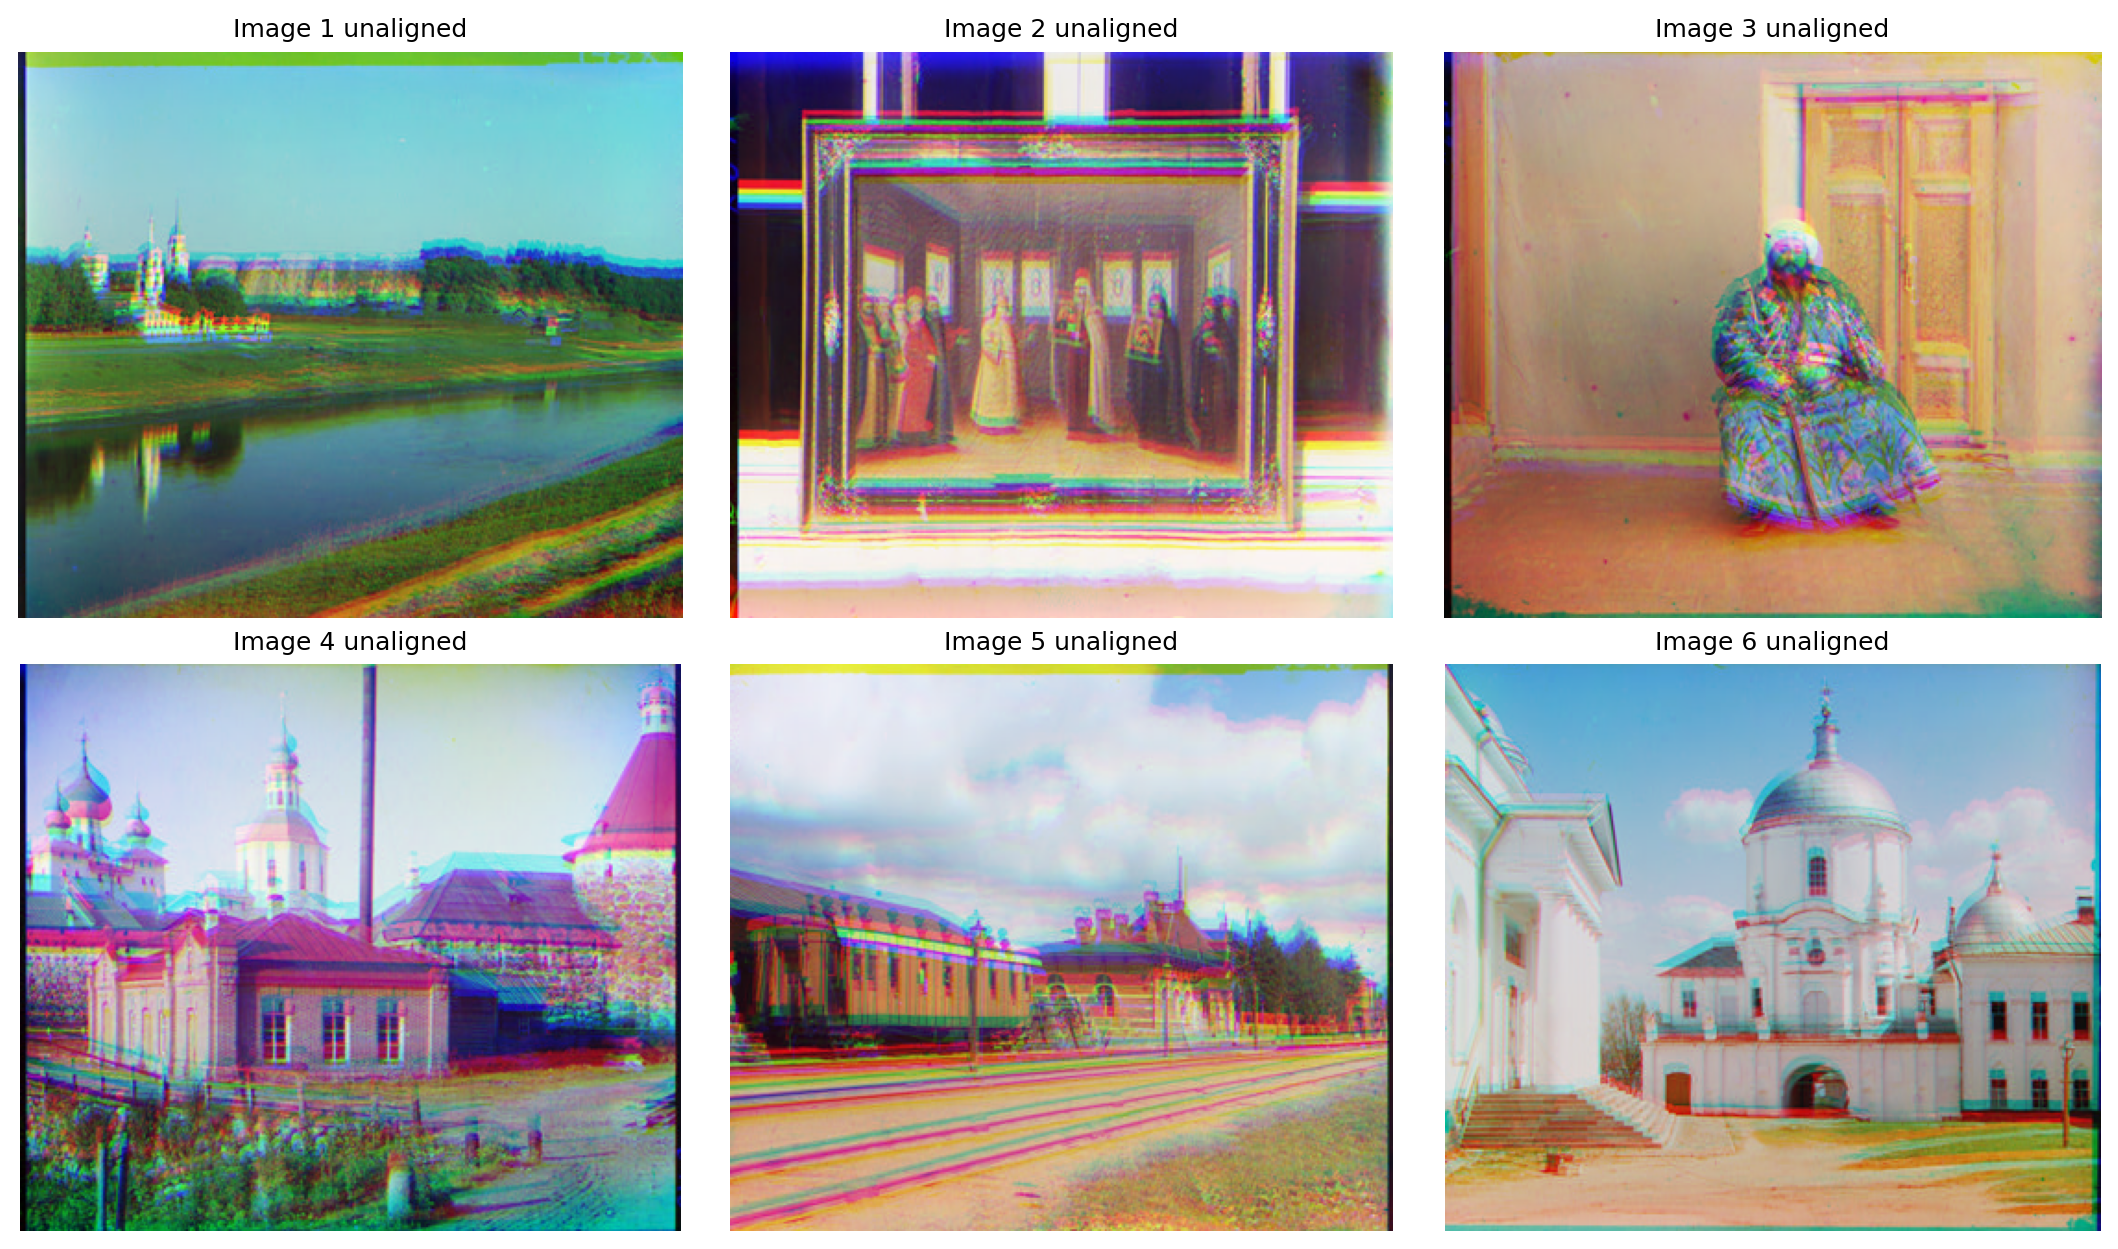
\includegraphics[width=0.95\linewidth]{student_response/figures/part1_grid_unaligned.png}
\caption{Part 1 baseline (unaligned channel stacking) for all 6 images.}
\label{fig:p1-unaligned}
\end{figure}

\begin{figure}[htbp]
\centering
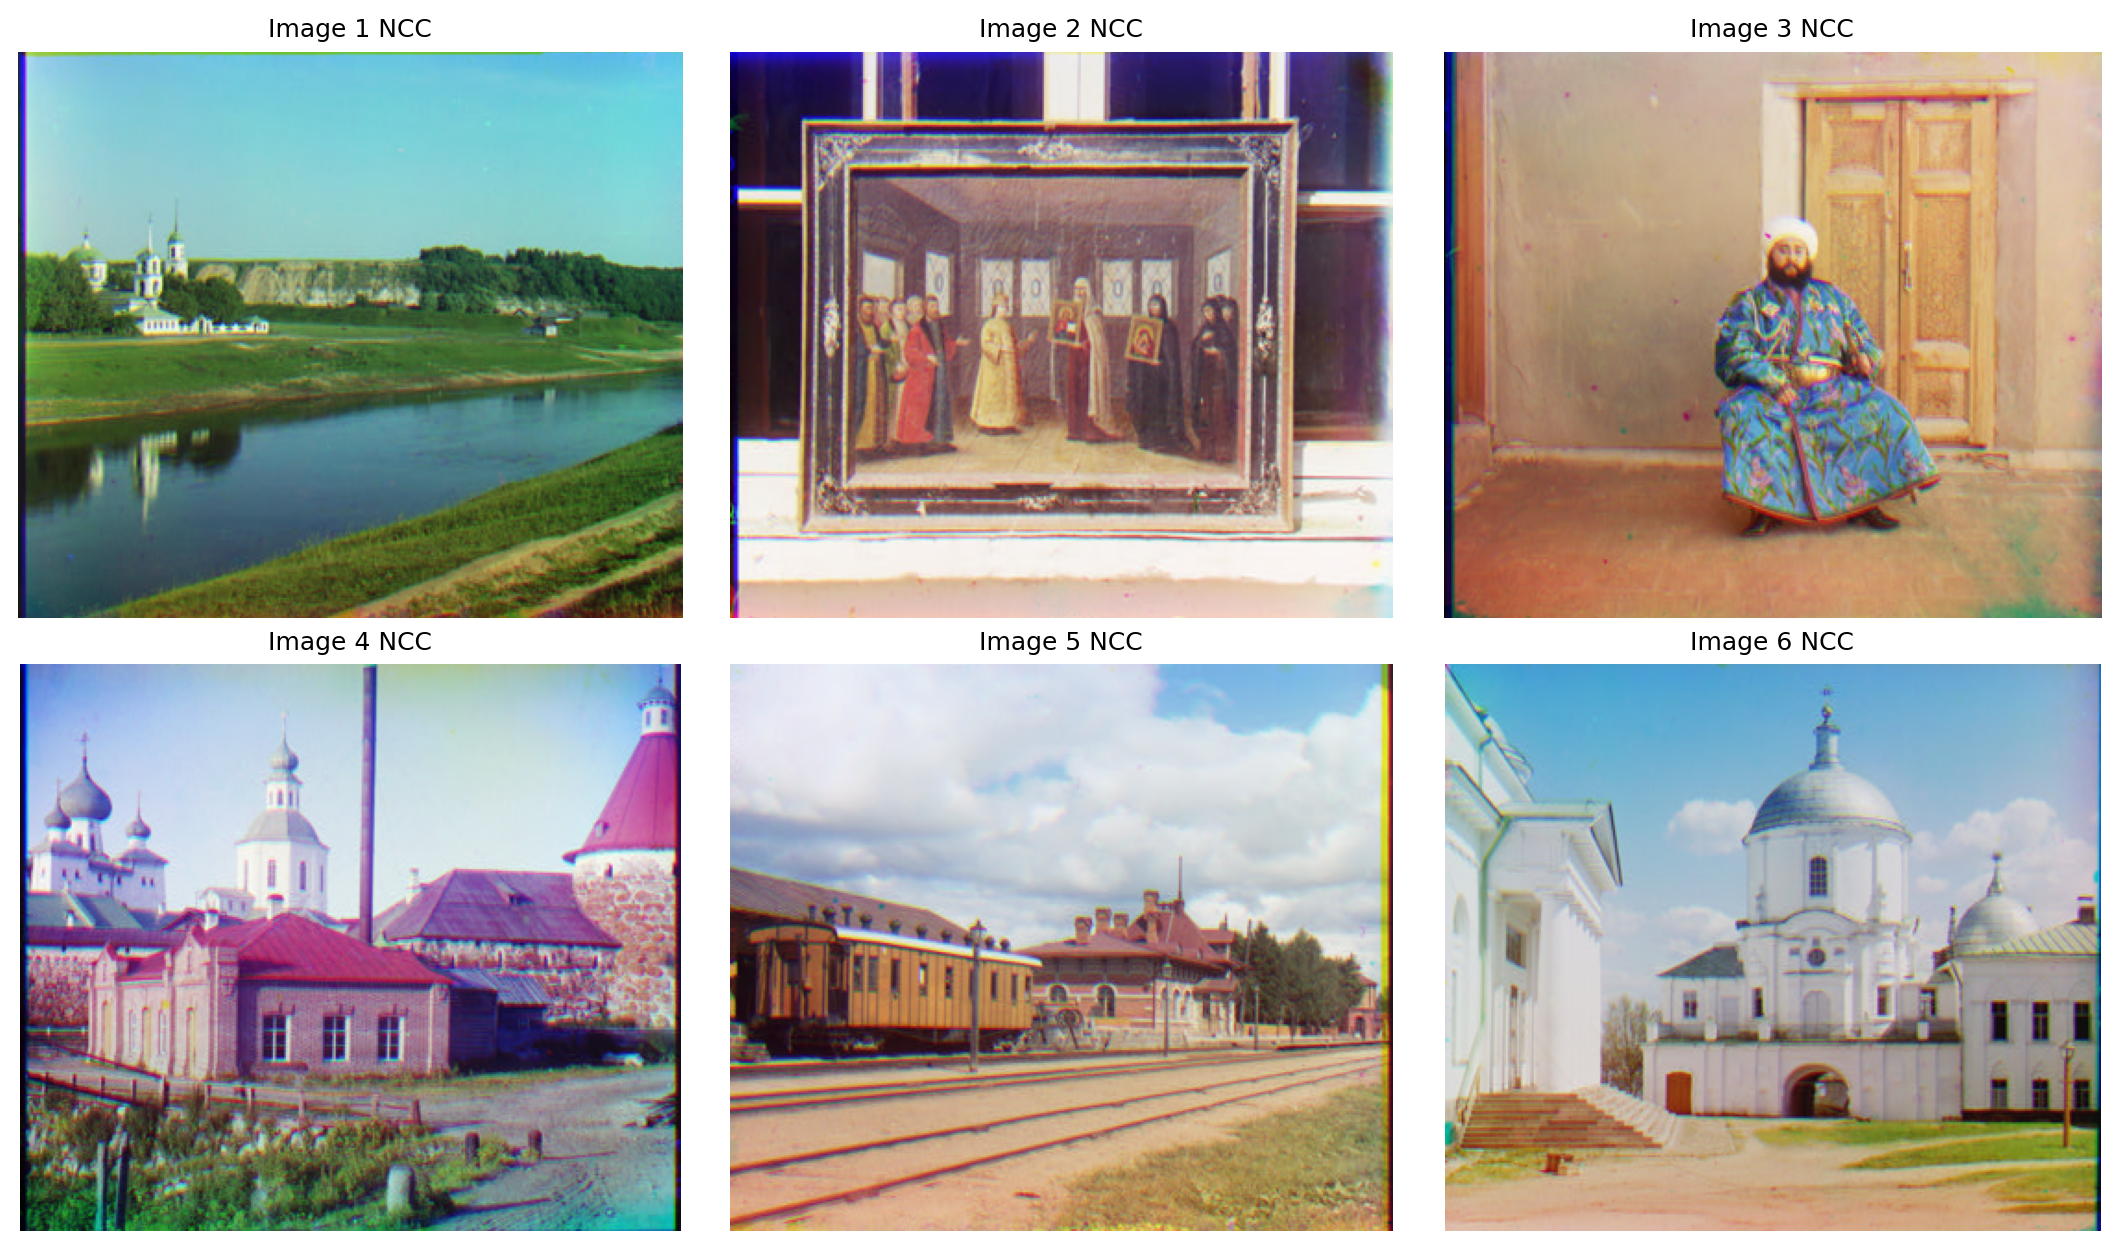
\includegraphics[width=0.95\linewidth]{student_response/figures/part1_grid_ncc_aligned_DIFF.png}
\caption{Part 1 aligned outputs with NCC.}
\label{fig:p1-ncc}
\end{figure}

\begin{figure}[htbp]
\centering
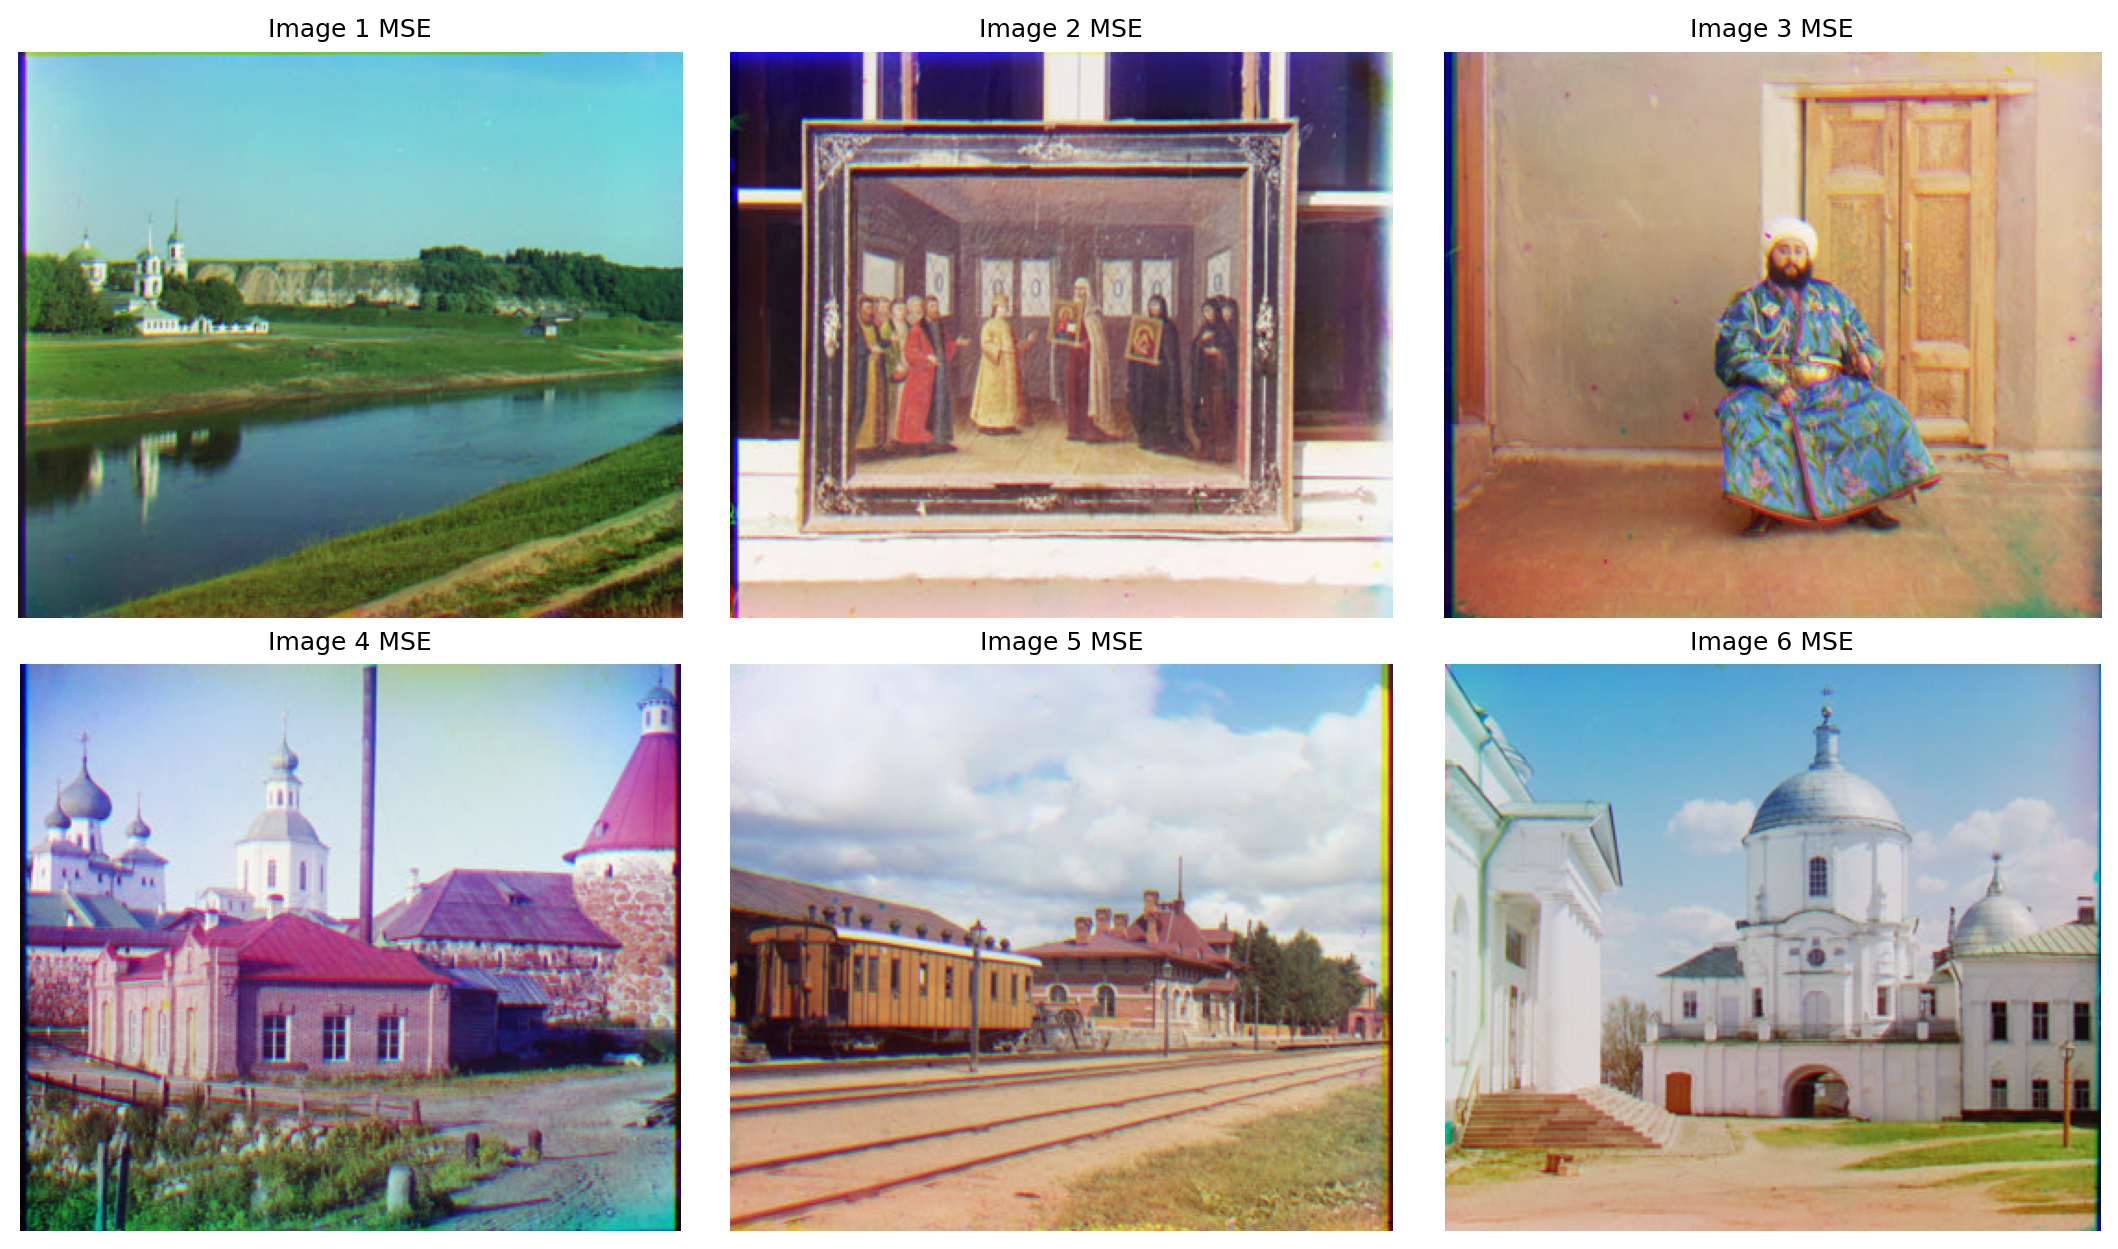
\includegraphics[width=0.95\linewidth]{student_response/figures/part1_grid_mse_aligned_DIFF.png}
\caption{Part 1 aligned outputs with MSE.}
\label{fig:p1-mse}
\end{figure}

\clearpage

\subsection*{Part 1 Limitations, Findings, and Failure Cases}
\label{sec:p1-findings}
\begin{itemize}
\item A single global translation cannot fix perspective/non-rigid differences; some border fringing remains.
\item Low-texture channels (especially in image 6) make $B\rightarrow G$ sensitive to the chosen loss.
\item What worked well: edge-first + coarse-to-fine gave robust convergence with reasonable runtime.
\item What worked less well: pure translation model is structurally limited for difficult images.
\end{itemize}

\clearpage

\section*{Part 2: Scale-Space Blob Detection}
\label{sec:part2}

\subsection*{Detailed Mathematical Formulation}
\label{sec:p2-method}
Let $I(x,y)$ be grayscale input and $G(x,y;\sigma)$ be a Gaussian kernel with scale $\sigma$.
The (unnormalized) LoG operator is:
\begin{equation}
\label{eq:p2-log}
\nabla^2 G(x,y;\sigma)=\frac{\partial^2 G}{\partial x^2}+\frac{\partial^2 G}{\partial y^2}.
\end{equation}
Scale-normalized LoG response at discrete scale $\sigma_i$ is:
\begin{equation}
\label{eq:p2-response}
R(x,y,\sigma_i)=\left(\sigma_i^2\,\big(\nabla^2 G_{\sigma_i} * I\big)(x,y)\right)^2,
\quad \sigma_i=\sigma_0 k^i.
\end{equation}
I square the response so both bright-on-dark and dark-on-bright blobs produce positive peaks. Blob radius is mapped by:
\begin{equation}
\label{eq:p2-radius}
r_i=\sqrt{2}\,\sigma_i.
\end{equation}

To reduce compute, instead of increasing kernel size aggressively at each scale, the implementation downsamples images through the pyramid and upsamples responses to a common resolution for 3D NMS. This approximates large-scale filtering with lower convolution cost.

\subsection*{Algorithm Overview and Implementation Stages}
\label{sec:p2-overview}
Pipeline stages:
\begin{enumerate}
\item Convert RGB image to grayscale (or grayscale read directly).
\item Build LoG kernel(s) and generate scale-space responses.
\item Apply 3D non-maximum suppression in $(x,y,\sigma)$.
\item Apply profile-specific thresholding and pruning stages.
\item Convert surviving scale index to circle radius and render circles.
\item Save outputs and detailed logs (stage counts, runtimes, detection json).
\end{enumerate}

For non-exact profiles, filtering stages are logged as:
\texttt{raw\_candidates} $\rightarrow$ \texttt{after\_score\_keep} $\rightarrow$ \texttt{after\_border\_soft} $\rightarrow$ \texttt{after\_border\_hard} $\rightarrow$ \texttt{after\_quality} $\rightarrow$ \texttt{after\_iou\_nms} $\rightarrow$ \texttt{final\_count}.

\subsection*{Hyperparameters, Their Meaning, and Why Chosen}
\label{sec:p2-hyperparams}
\begin{table}[htbp]
\centering
\scriptsize
\begin{tabular}{l|l|l}
\hline
Parameter & Meaning & Chosen values / rationale\\
\hline
$\sigma_0$ & Base scale & 1.6 (standard LoG starting scale for natural images)\\
$k$ & Scale multiplier & 1.2 (dense enough sampling across scales)\\
$n$ & Number of scales & 12 (non-exact), 15 (exact profile)\\
\texttt{ksize} & LoG kernel size & 9 for non-exact; dynamic for exact (from scale)\\
\texttt{q\_scale}, \texttt{q\_global} & Quantile thresholds & tuned for balanced/high\_recall precision-recall control\\
\texttt{abs\_threshold} & Absolute threshold & used by dense/exact for high-sensitivity detection\\
\texttt{iou\_thresh}, \texttt{dist\_overlap} & Circle deduplication controls & reduce duplicates while preserving nearby valid blobs\\
\texttt{border margins} & Border suppression & reduce frame-edge artifacts\\
\texttt{quality\_min} & Prominence filtering & remove weak peaks in noisy textured regions\\
\hline
\end{tabular}
\caption{Key hyperparameters and interpretation for Part 2 profiles.}
\label{tab:p2-hyperparams}
\end{table}

\subsection*{Computation Tables and Metric Discussion}
\label{sec:p2-metrics}
Overall proxy TP/FP/FN (silver-GT consensus) from \texttt{part2\_profile\_proxy\_overall.csv}:
\begin{table}[htbp]
\centering
\small
\begin{tabular}{l|r|r|r|r|r|r|r}
\hline
Profile & TP & FP & FN & Precision & Recall & F1 & Mean runtime (s)\\
\hline
balanced & 73 & 10 & 241 & 0.8795 & 0.2325 & 0.3678 & 0.9290\\
high\_recall & 130 & 11 & 184 & 0.9220 & 0.4140 & 0.5714 & 0.9445\\
dense & 314 & 364 & 0 & 0.4631 & 1.0000 & 0.6331 & 0.6728\\
exact & 275 & 3297 & 39 & 0.0770 & 0.8758 & 0.1415 & 39.6597\\
\hline
\end{tabular}
\caption{Overall proxy evaluation.}
\label{tab:p2-overall}
\end{table}

Stage-cost summary from latest rows in \texttt{part2\_blob\_runs.csv}:
\begin{table}[htbp]
\centering
\small
\begin{tabular}{l|r|r|r|r}
\hline
Profile & Mean raw candidates & Mean after IoU-NMS & Mean final count & Mean runtime (s)\\
\hline
balanced & 44.75 & 22.25 & 20.75 & 0.9290\\
high\_recall & 49.25 & 36.75 & 35.25 & 0.9445\\
dense & 262.25 & 172.00 & 169.50 & 0.6728\\
exact & 2877390.00 & 893.00 & 893.00 & 39.6597\\
\hline
\end{tabular}
\caption{Average candidate flow and runtime by profile (4 images).}
\label{tab:p2-stage-cost}
\end{table}

Interpretation:
\begin{itemize}
\item \textbf{balanced}: best precision, lowest recall; suitable when false positives must be minimal.
\item \textbf{high\_recall}: better recall while keeping precision high; good default for visual quality.
\item \textbf{dense}: highest proxy F1 due to full recall, but with many extra detections.
\item \textbf{exact}: very high recall but overwhelming FP and runtime; useful mainly as an upper-bound detector.
\end{itemize}

\clearpage

\subsection*{Special Tricks That Helped Part 2}
\label{sec:p2-tricks}
The following implementation details materially improved results:
\begin{enumerate}
\item \textbf{Scale normalization ($\sigma^2$)} to keep responses comparable across scales.
\item \textbf{Soft border thresholding} so near-boundary peaks need stronger evidence.
\item \textbf{Two-step circle deduplication} (IoU NMS + distance-overlap suppression).
\item \textbf{Profile-based operating modes} to expose precision/recall/runtime tradeoff explicitly.
\item \textbf{Detailed stage logging} to diagnose where detections are removed.
\end{enumerate}

\subsection*{Part 2 Limitations and Findings}
\label{sec:p2-findings}
\begin{itemize}
\item Silver-GT proxy metrics are comparative only; they are not absolute human-labeled accuracy.
\item Exact profile can become computationally heavy and over-detective on highly textured images.
\item Dense profile maximizes recall/F1 proxy but can clutter output with false positives.
\item High\_recall profile gave the best practical visual balance in this dataset.
\end{itemize}

\subsection*{Automatic TP/FP/FN Generation from Main Script}
\label{sec:p2-repro}
I integrated proxy evaluation directly into \texttt{main\_p2.py}. Running
\begin{itemize}
\item \texttt{python main\_p2.py -i all --run\_proxy\_eval}
\end{itemize}
now runs all four profiles and writes:
\texttt{part2\_profile\_proxy\_per\_image.csv}, \texttt{part2\_profile\_proxy\_overall.csv},
\texttt{part2\_profile\_proxy\_eval.md}, \texttt{part2\_profile\_proxy\_eval.json}.

\begin{figure}[htbp]
\centering
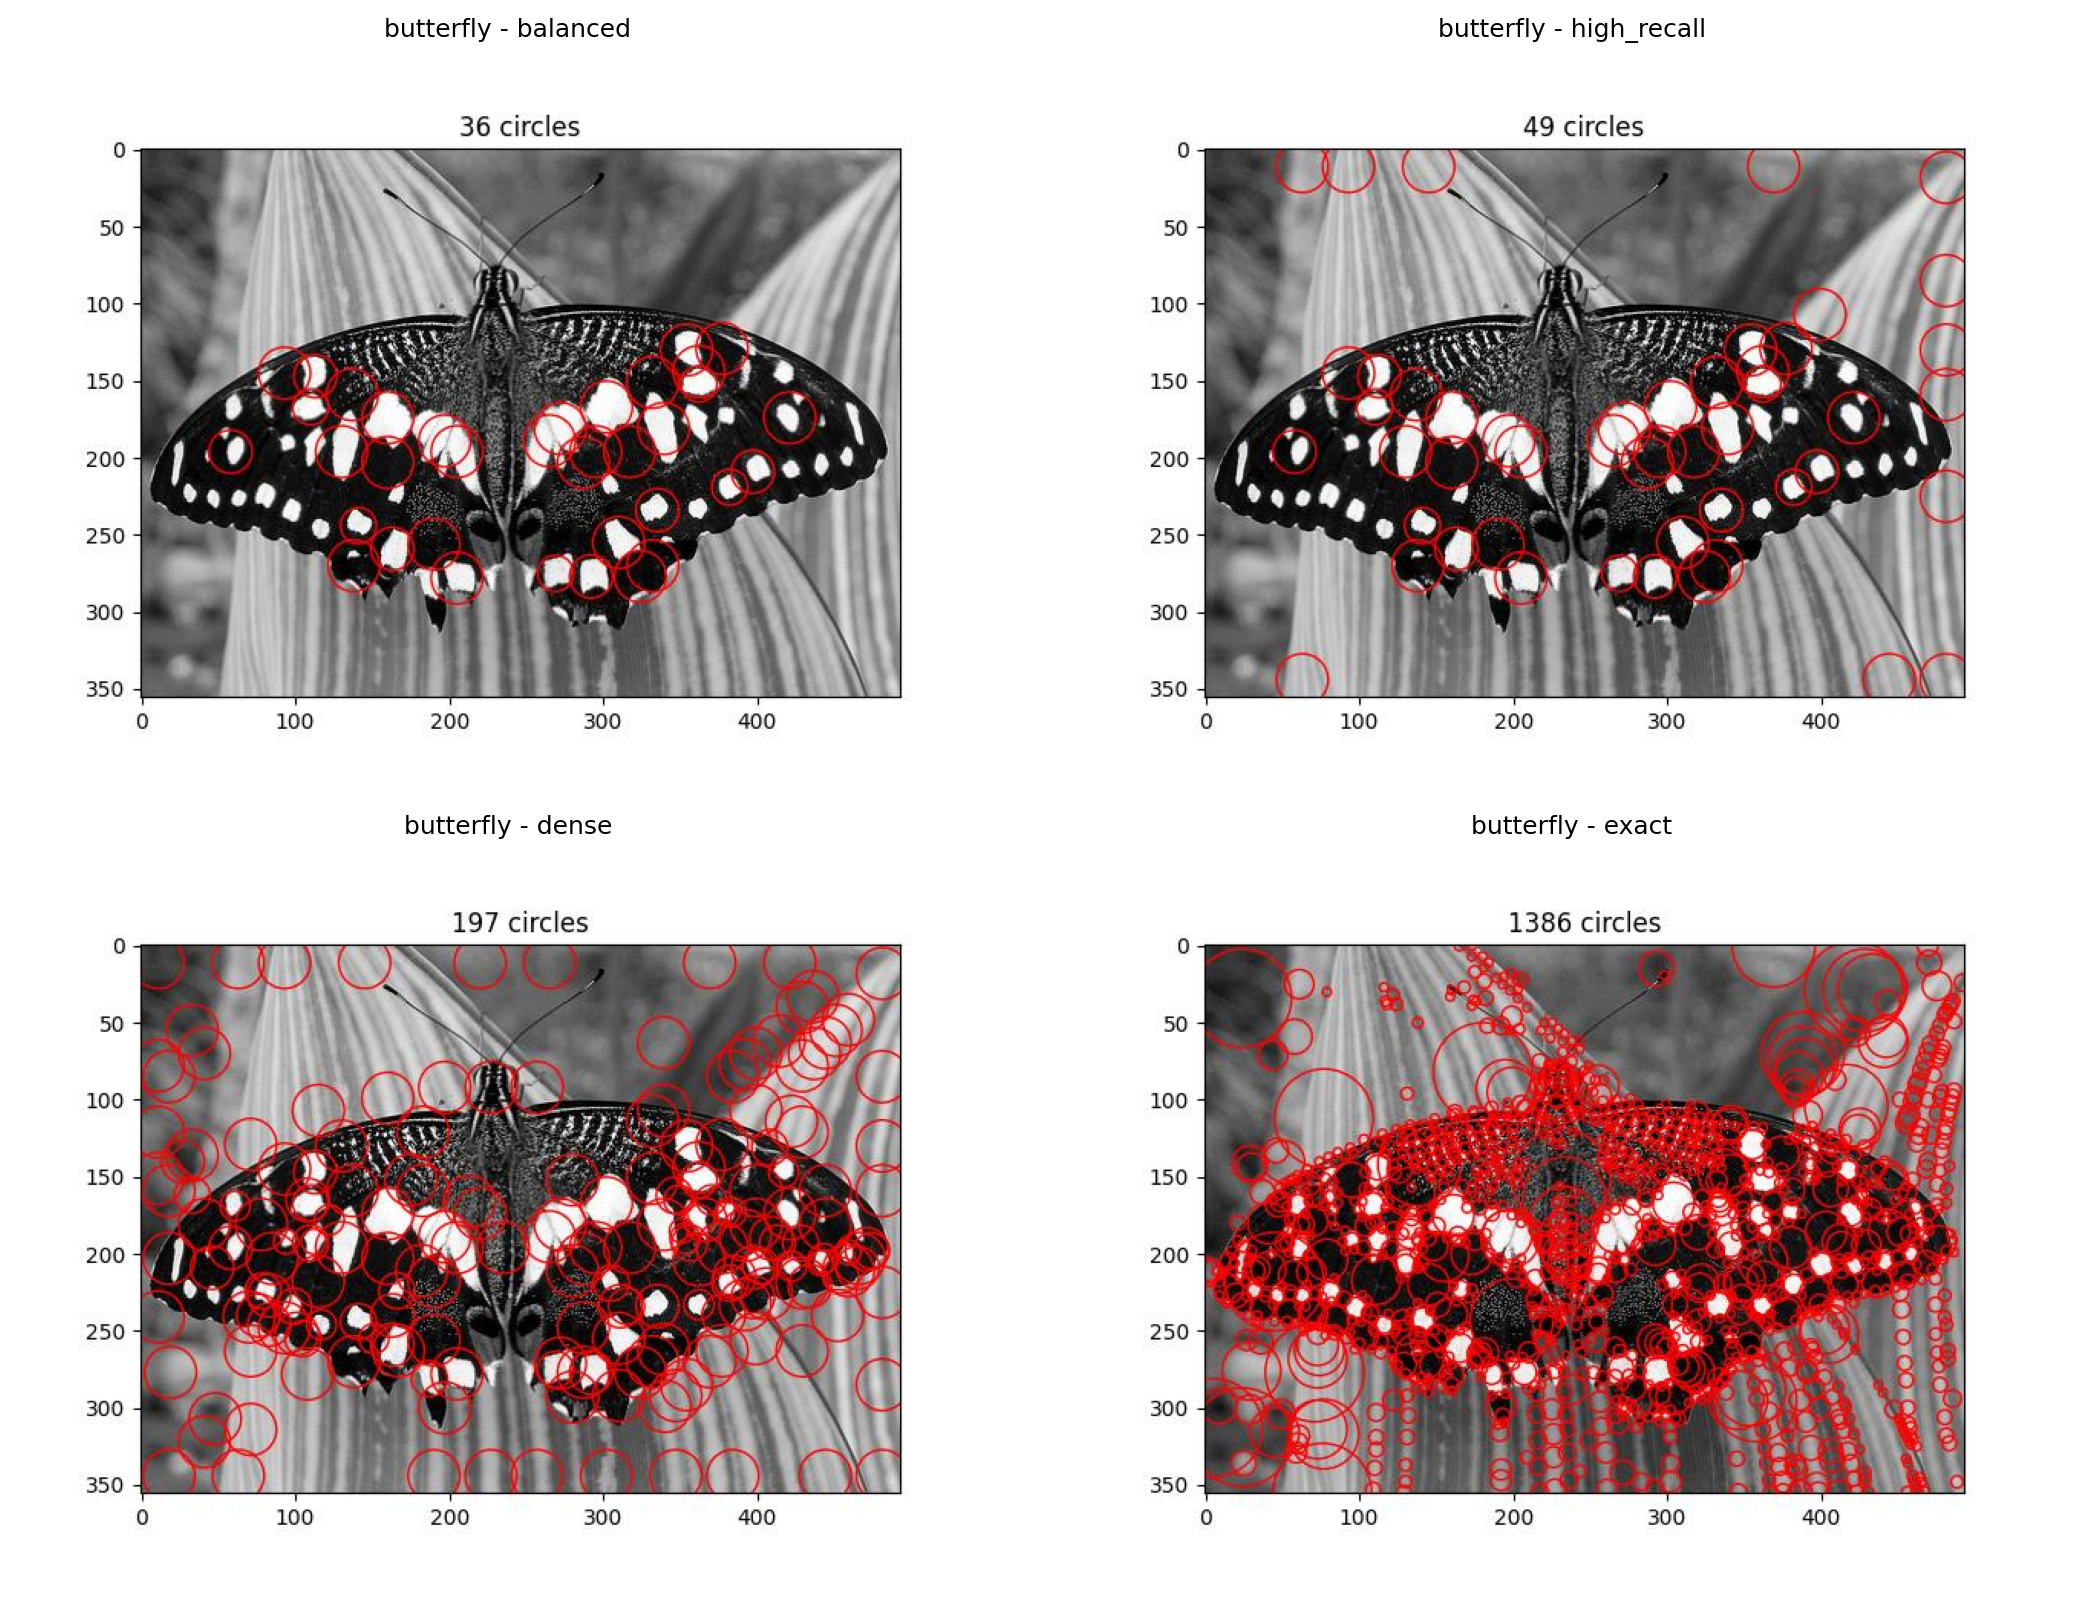
\includegraphics[width=0.93\linewidth]{student_response/figures/part2_profile_compare_butterfly.png}
\caption{Profile comparison on butterfly (balanced, high\_recall, dense, exact).}
\label{fig:p2-prof-butterfly}
\end{figure}

\begin{figure}[htbp]
\centering
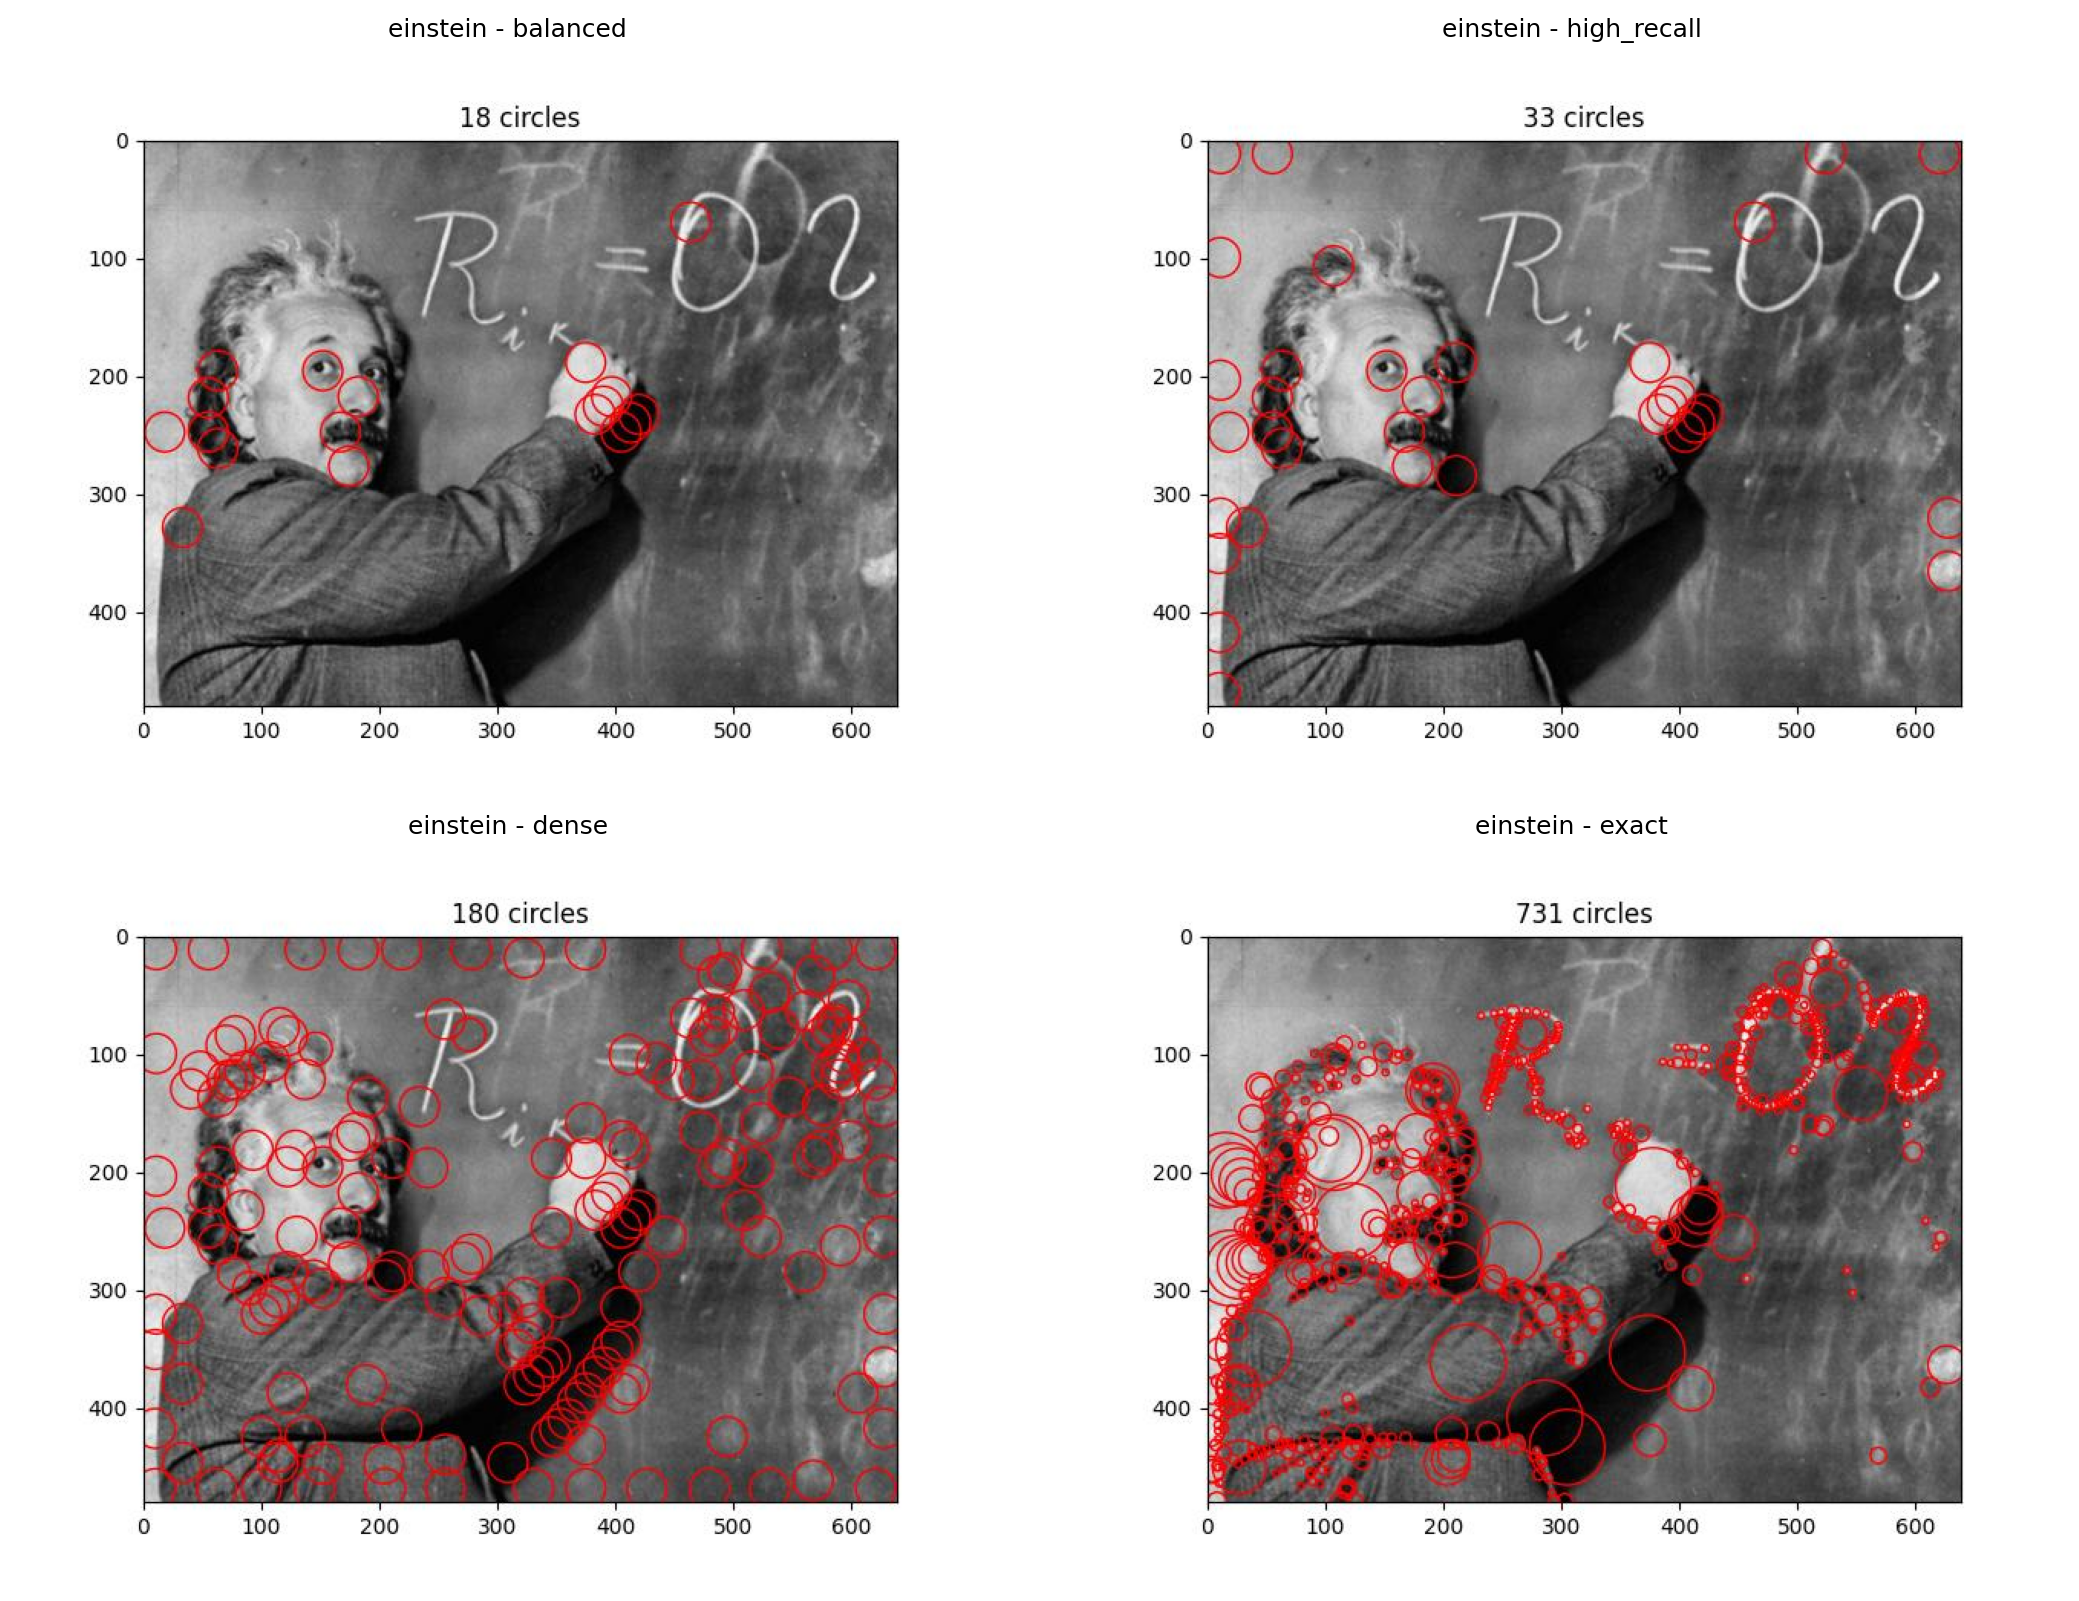
\includegraphics[width=0.93\linewidth]{student_response/figures/part2_profile_compare_einstein.png}
\caption{Profile comparison on einstein.}
\label{fig:p2-prof-einstein}
\end{figure}

\begin{figure}[htbp]
\centering
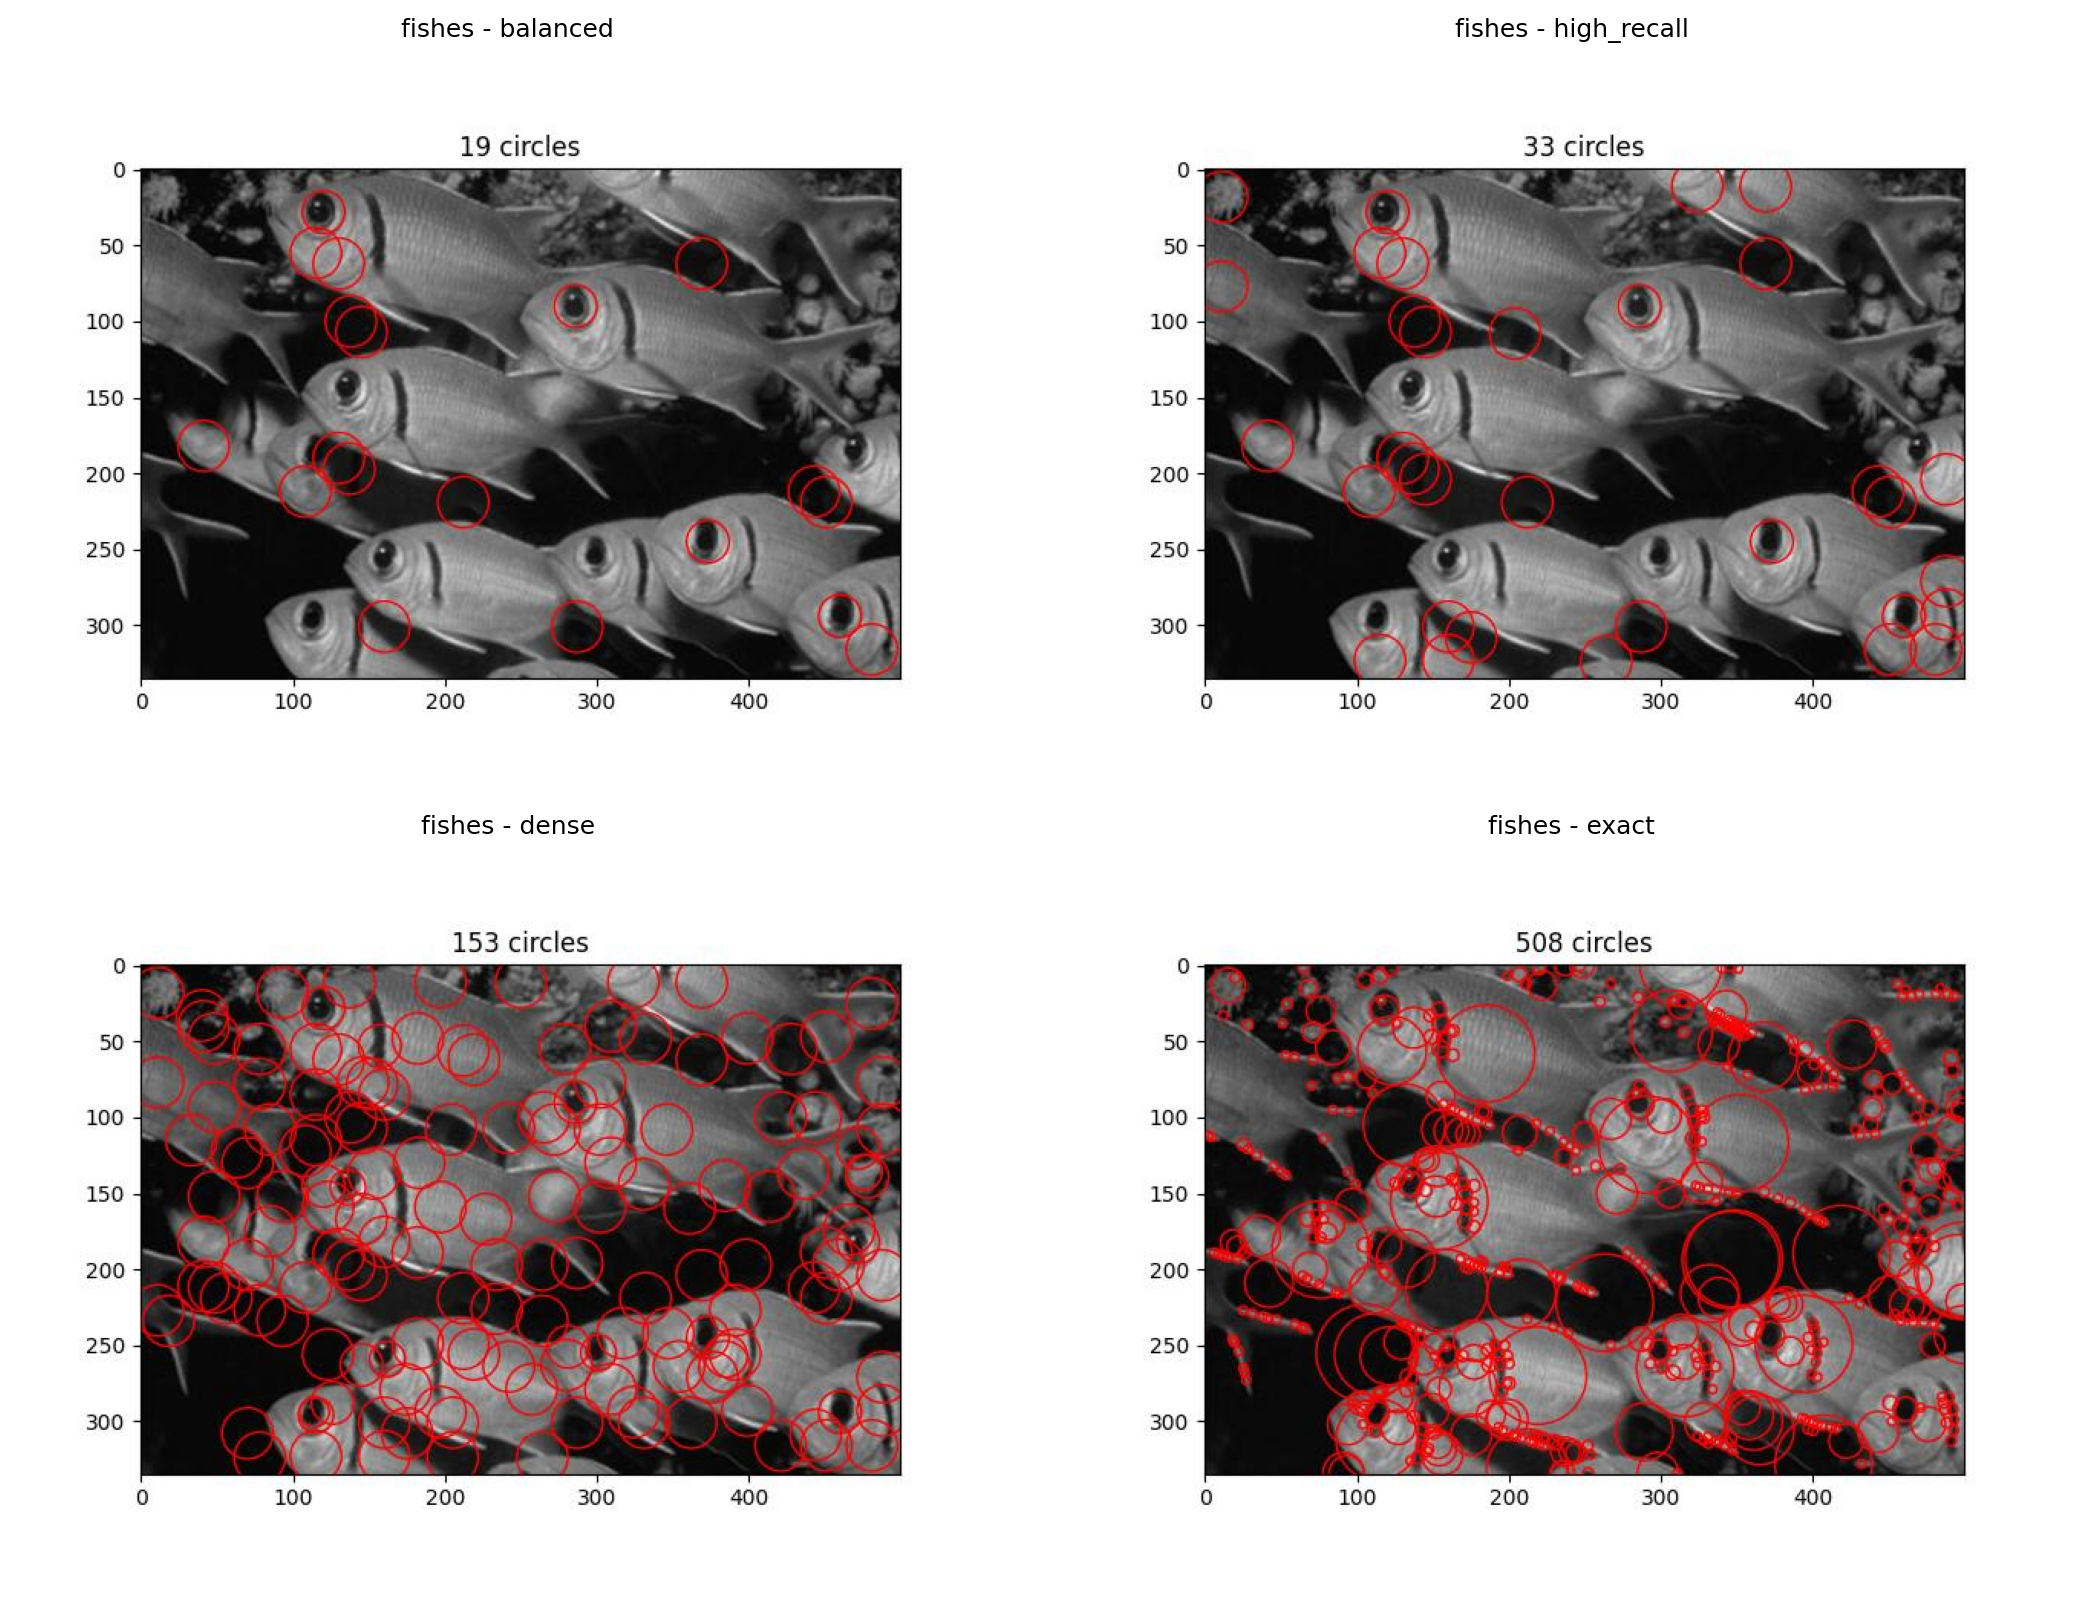
\includegraphics[width=0.93\linewidth]{student_response/figures/part2_profile_compare_fishes.png}
\caption{Profile comparison on fishes.}
\label{fig:p2-prof-fishes}
\end{figure}

\begin{figure}[htbp]
\centering
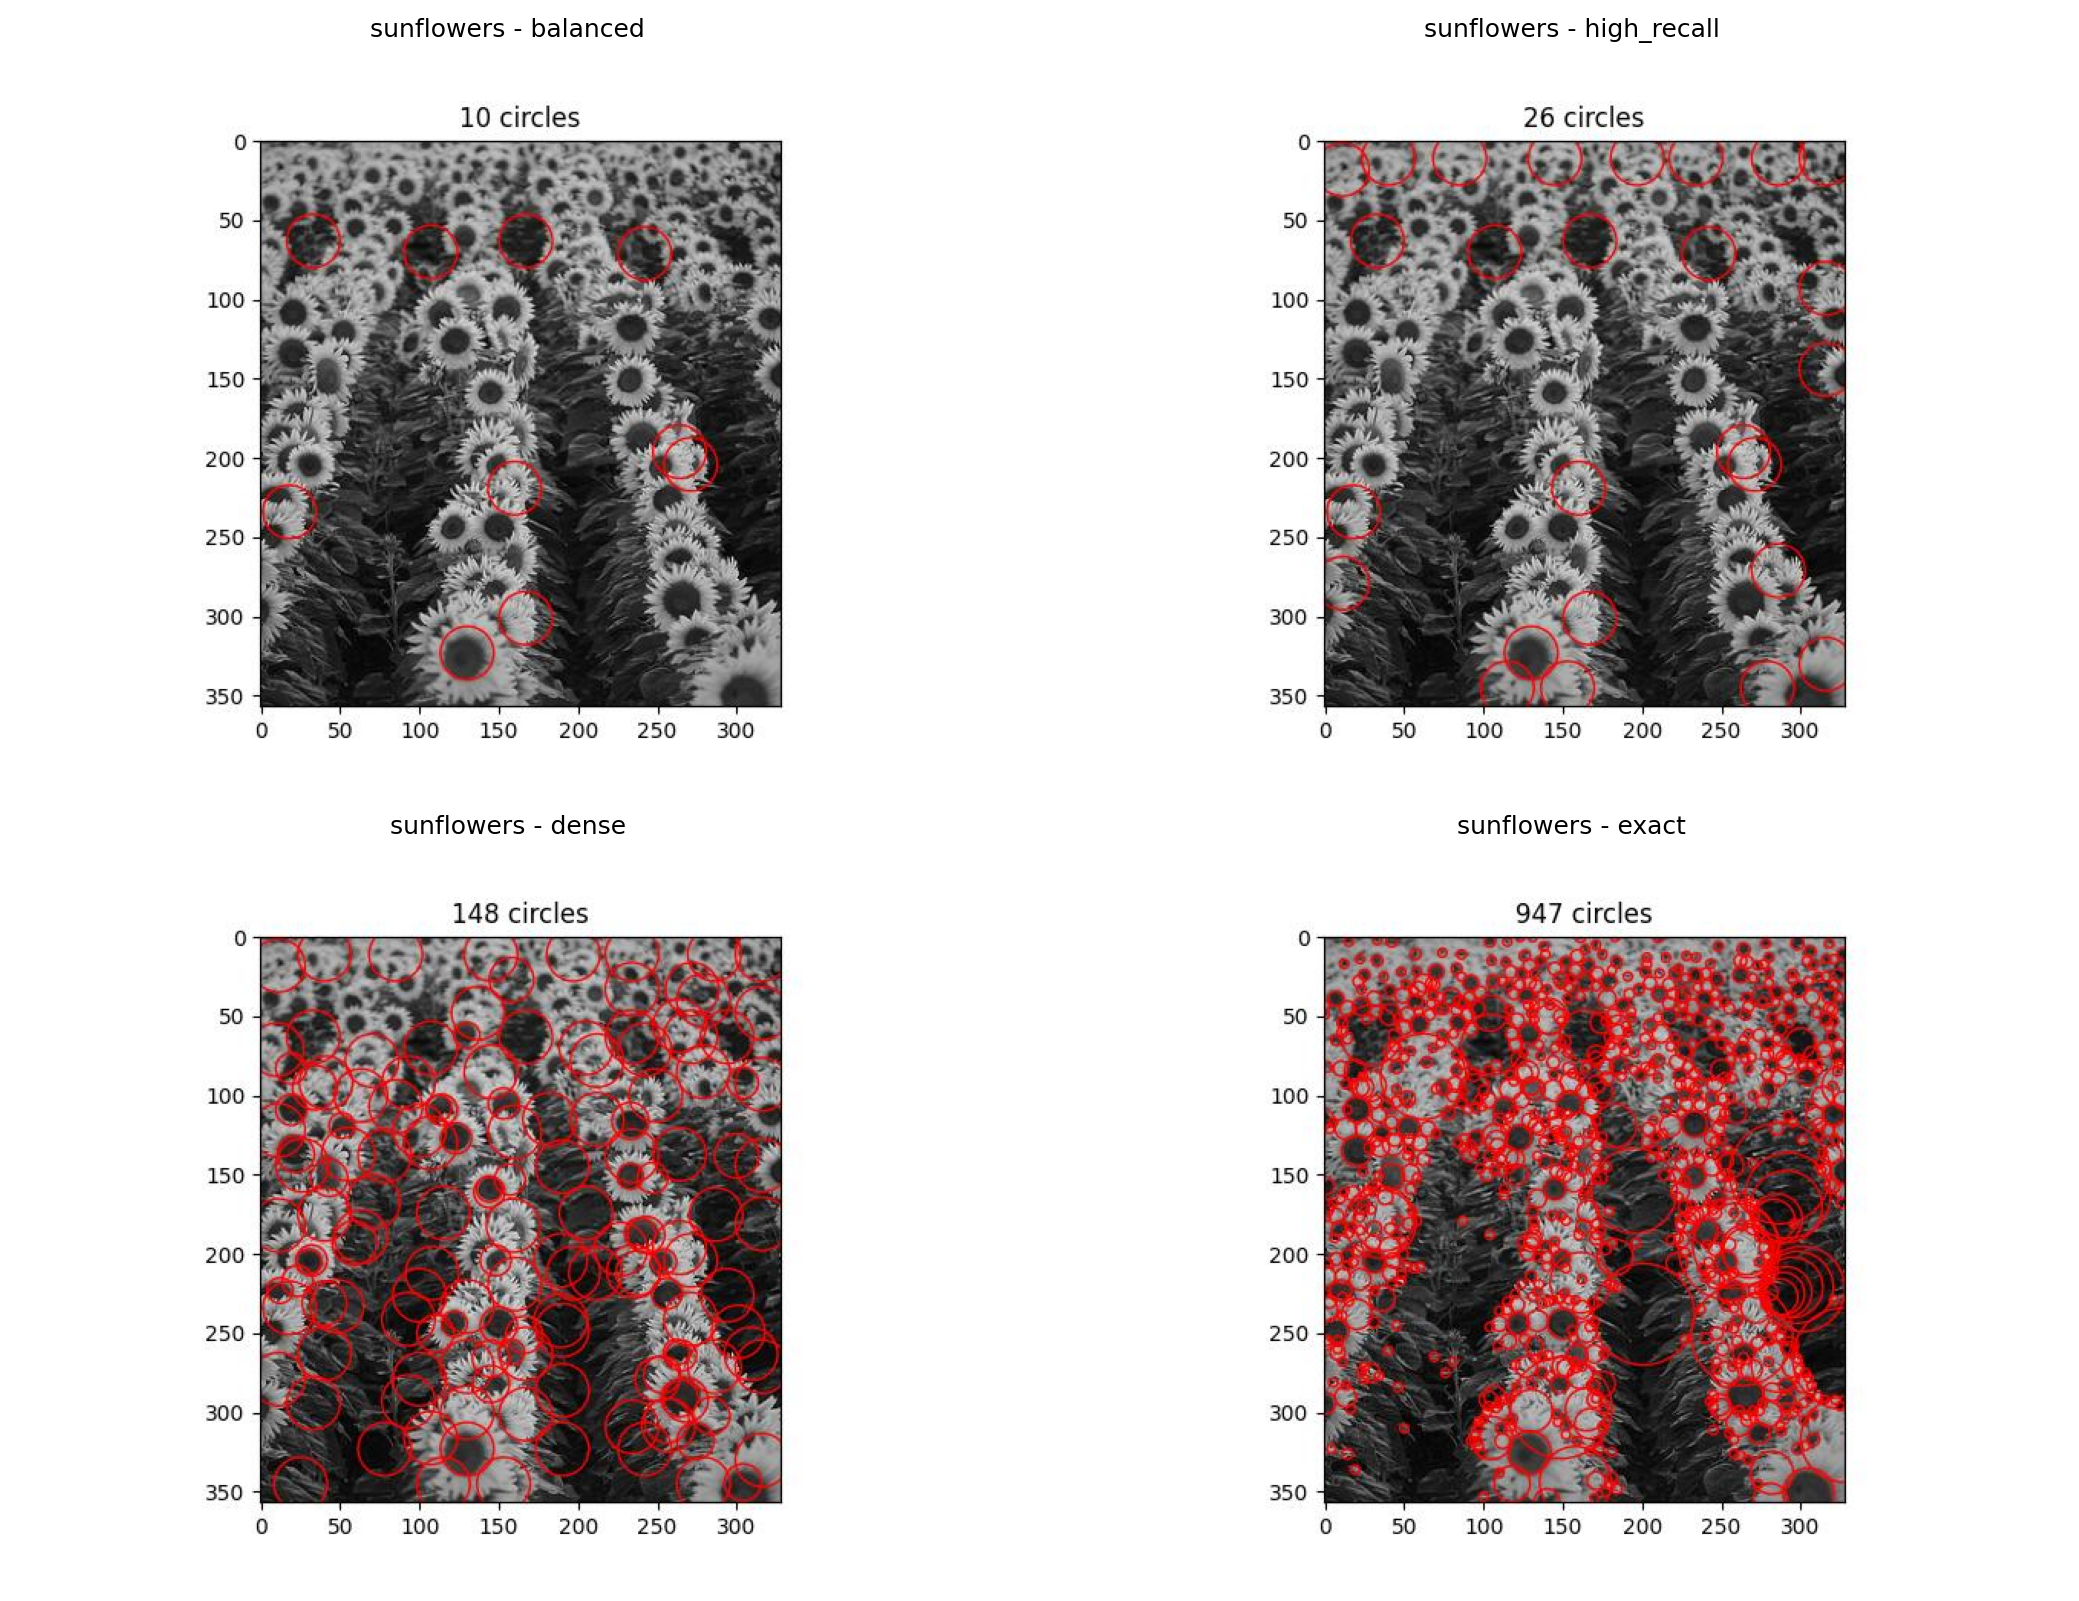
\includegraphics[width=0.93\linewidth]{student_response/figures/part2_profile_compare_sunflowers.png}
\caption{Profile comparison on sunflowers.}
\label{fig:p2-prof-sunflowers}
\end{figure}

\begin{figure}[htbp]
\centering
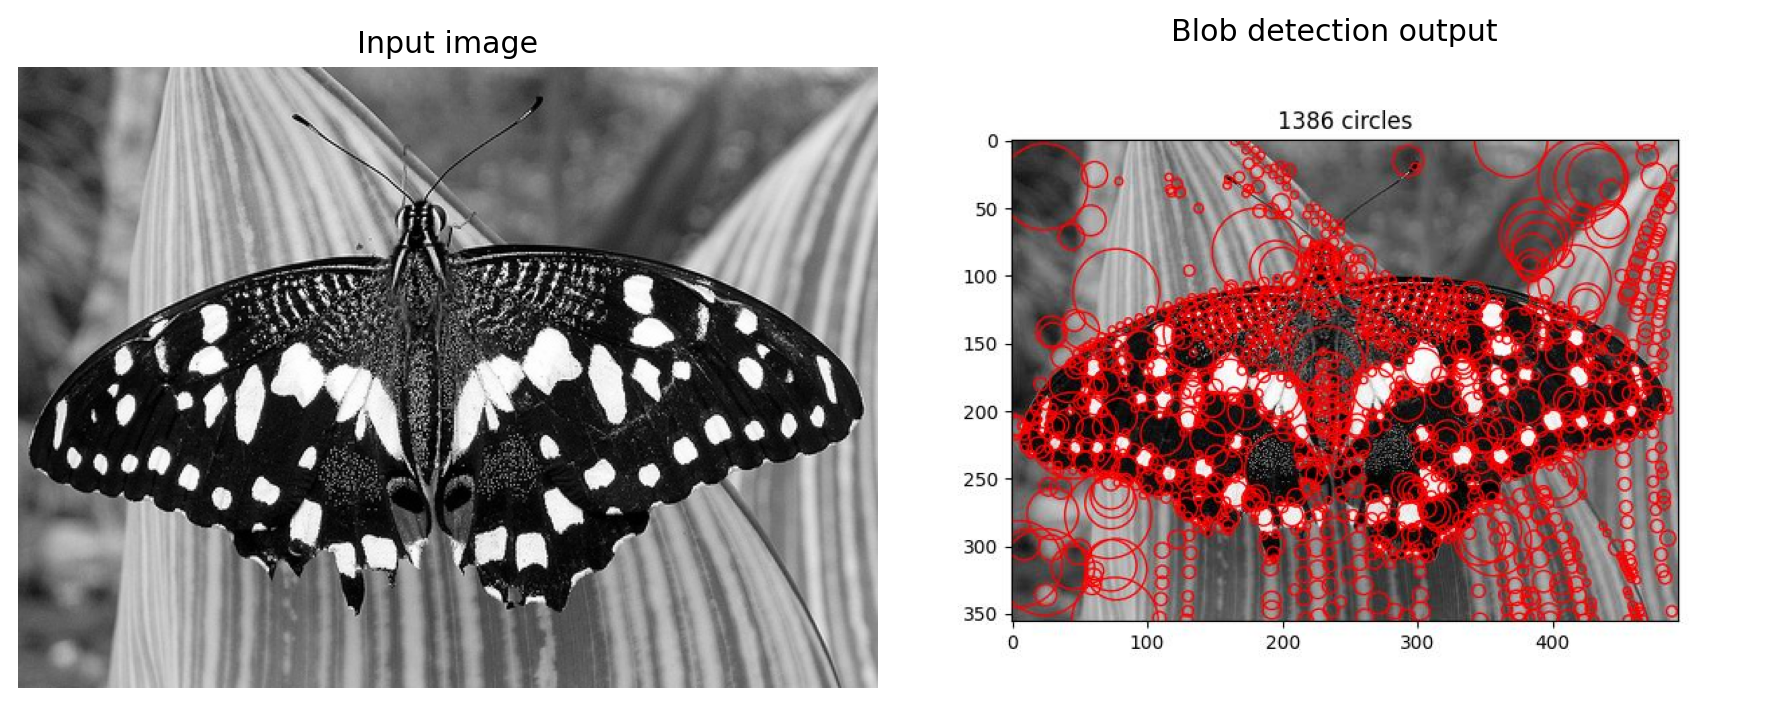
\includegraphics[width=0.95\linewidth]{student_response/figures/part2_before_after_butterfly.png}
\caption{Butterfly input vs blob output (final run).}
\label{fig:p2-before-after-butterfly}
\end{figure}

\begin{figure}[htbp]
\centering
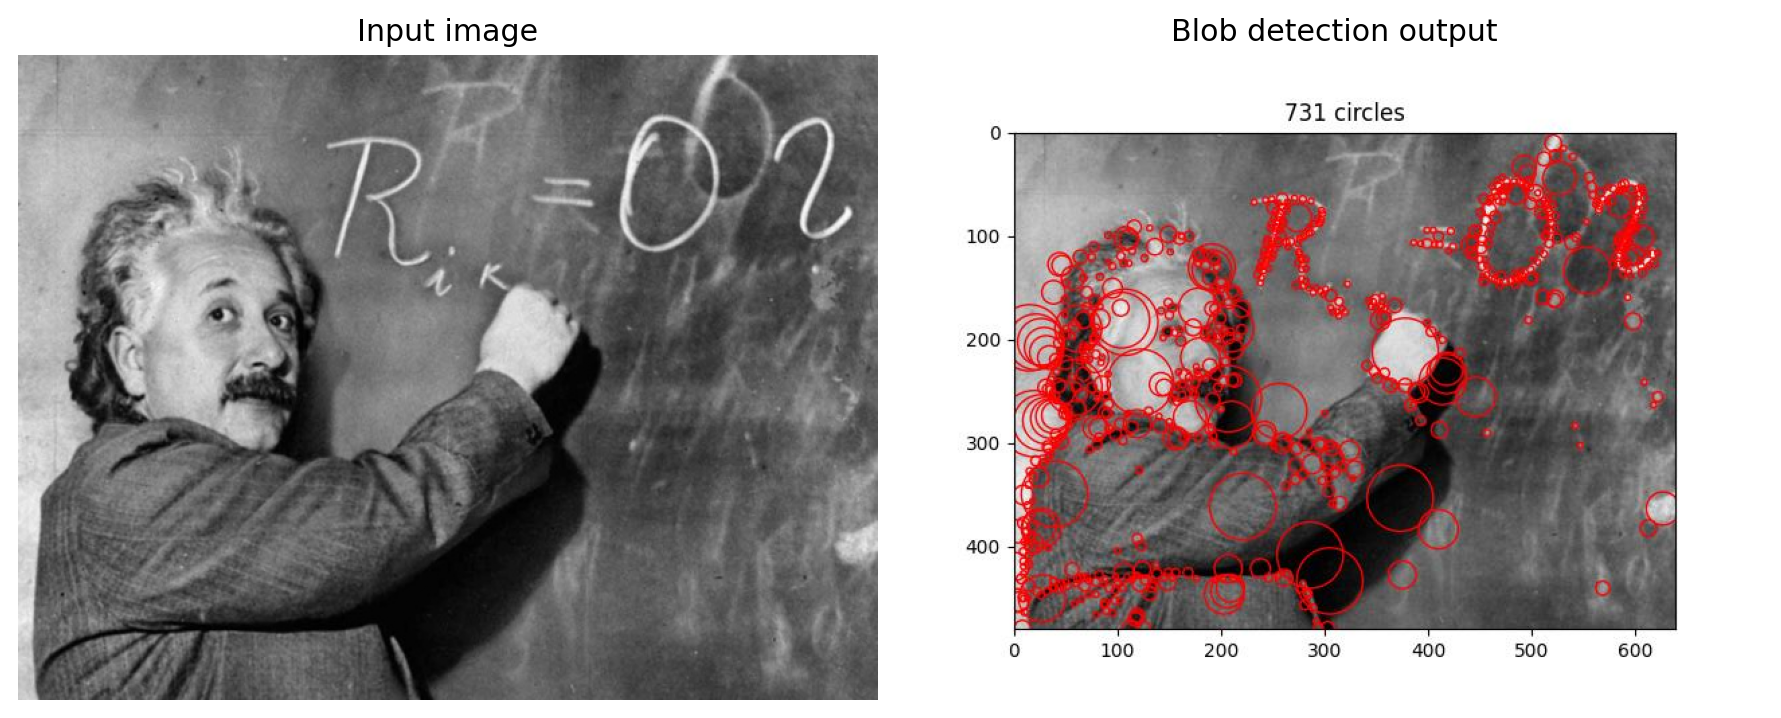
\includegraphics[width=0.95\linewidth]{student_response/figures/part2_before_after_einstein.png}
\caption{Einstein input vs blob output (final run).}
\label{fig:p2-before-after-einstein}
\end{figure}

\begin{figure}[htbp]
\centering
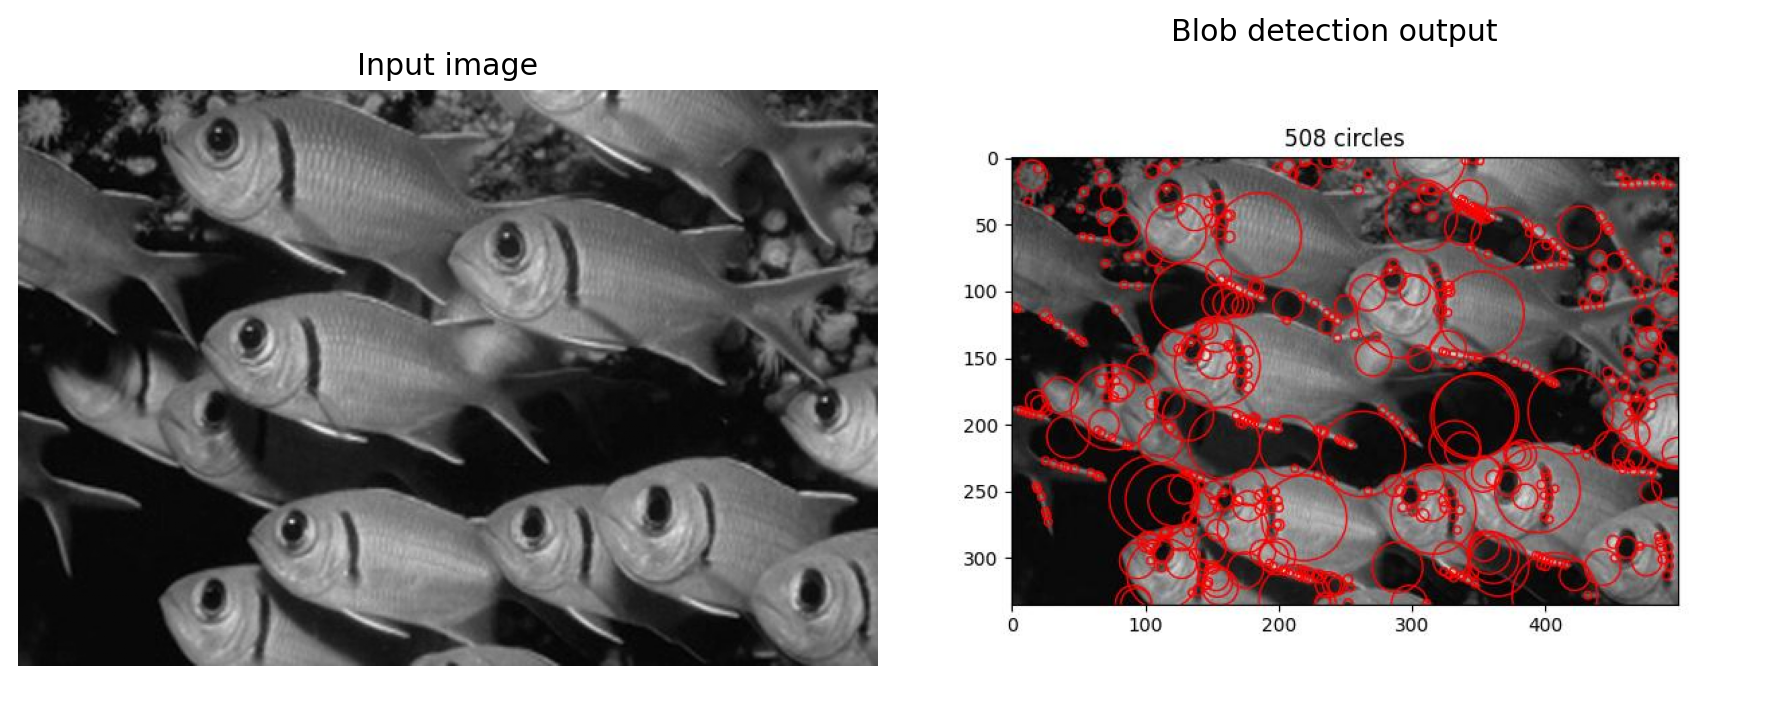
\includegraphics[width=0.95\linewidth]{student_response/figures/part2_before_after_fishes.png}
\caption{Fishes input vs blob output (final run).}
\label{fig:p2-before-after-fishes}
\end{figure}

\begin{figure}[htbp]
\centering
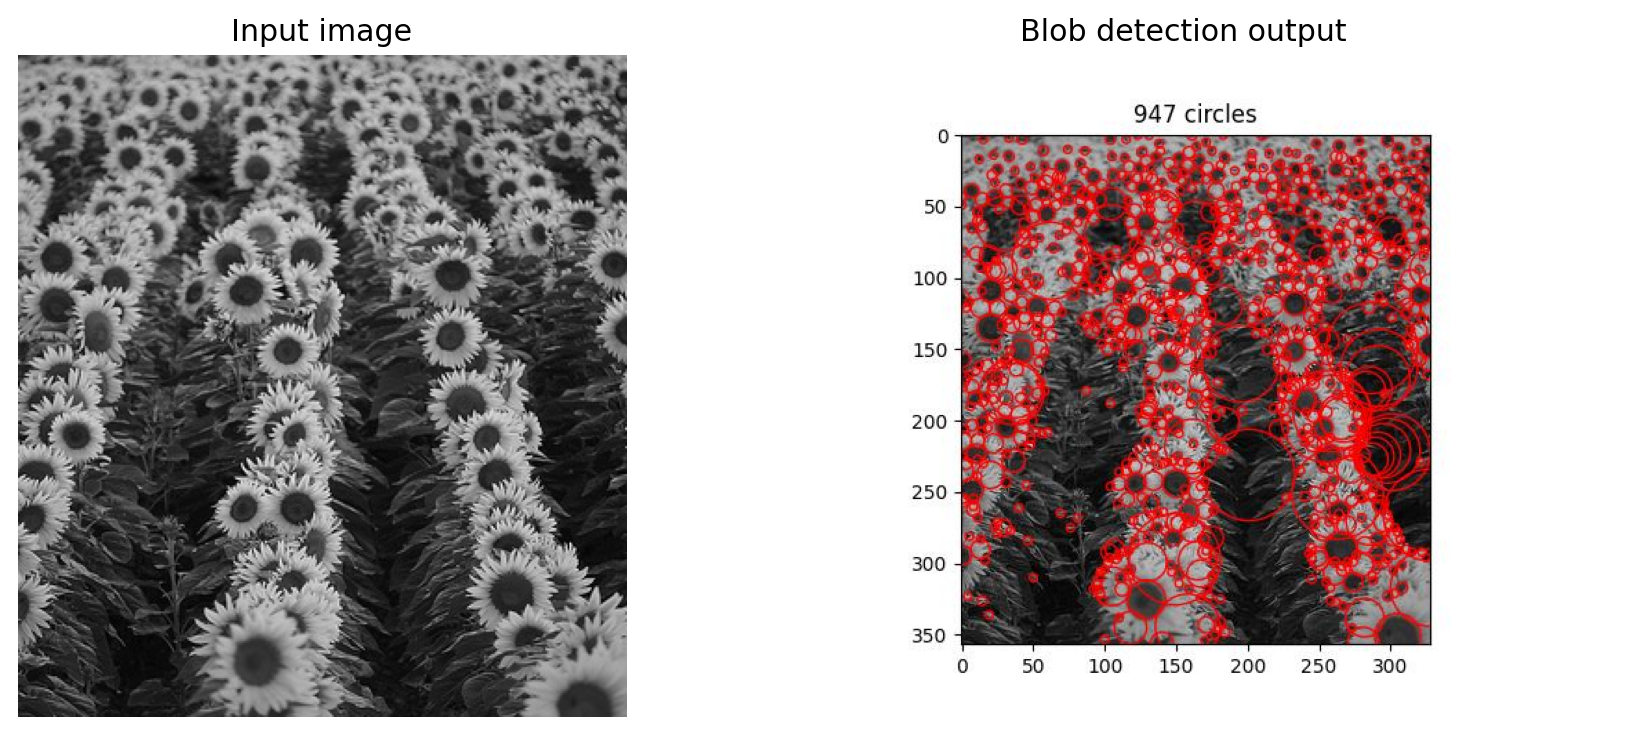
\includegraphics[width=0.95\linewidth]{student_response/figures/part2_before_after_sunflowers.png}
\caption{Sunflowers input vs blob output (final run).}
\label{fig:p2-before-after-sunflowers}
\end{figure}

\clearpage

\section*{Conclusion and Final Findings}
\label{sec:conclusion}
The final quantitative trend across profiles is summarized in Figure~\ref{fig:p2-aggregate}.
\begin{figure}[htbp]
\centering
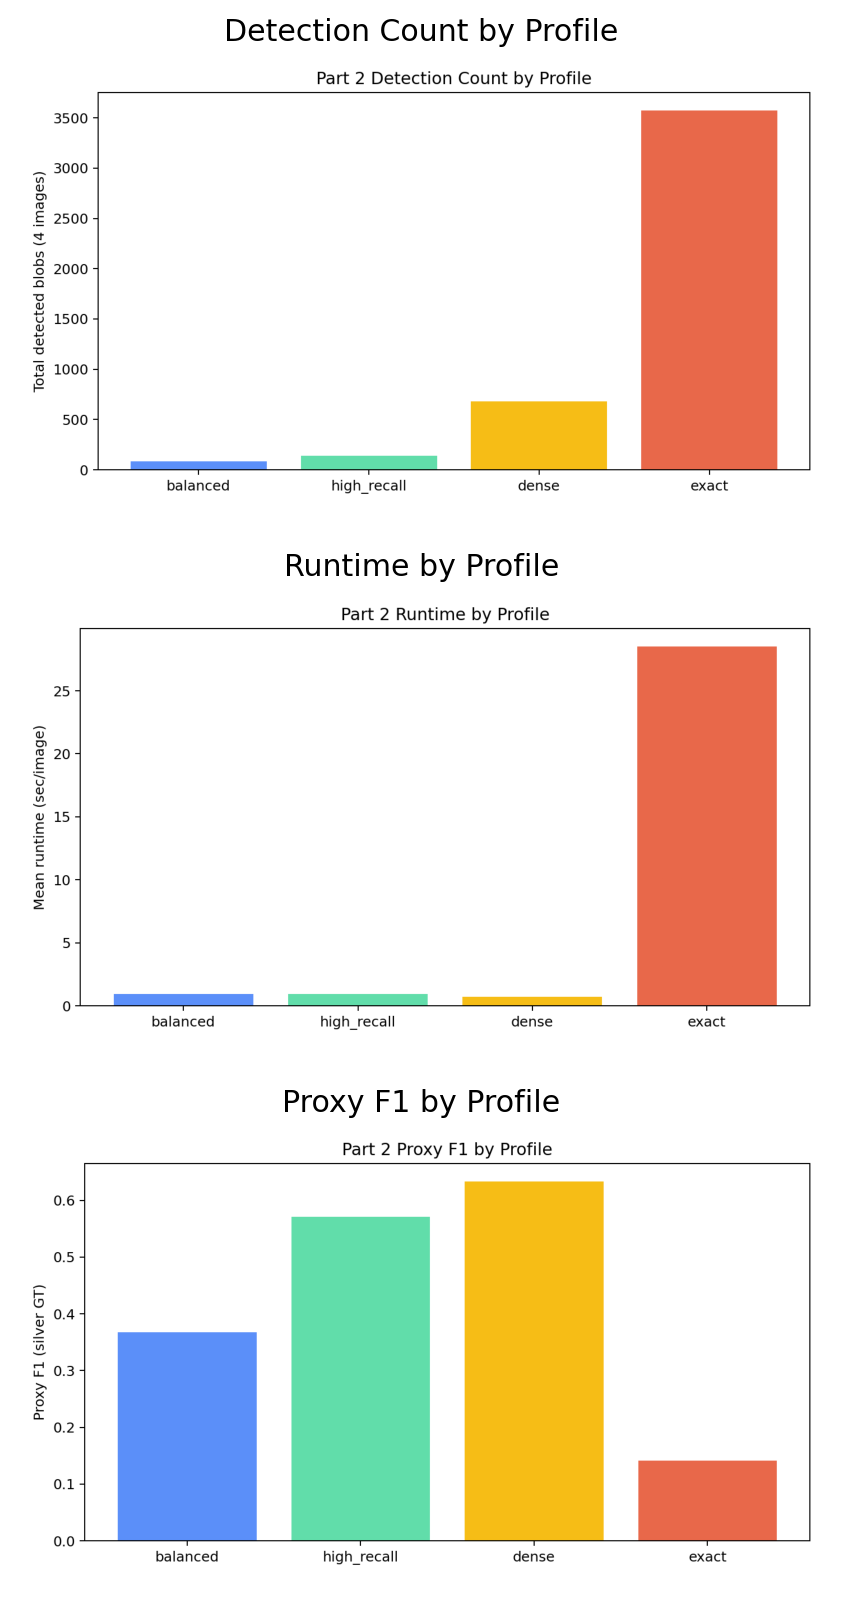
\includegraphics[height=0.78\textheight]{student_response/figures/part2_aggregate_vertical.png}
\caption{Aggregate trends by profile in a three-row readable layout: count, runtime, and proxy F1.}
\label{fig:p2-aggregate}
\end{figure}

\begin{itemize}
\item Part 1 achieved stable alignment on all six images with both NCC and MSE; shifts are largely similar but not identical.
\item Coarse-to-fine edge-first optimization was the key enabler for robust convergence.
\item Part 2 exhibits a clear precision-recall-runtime frontier across profiles.
\item Dense profile gives strongest proxy F1; high\_recall gives cleaner practical outputs; exact is an extreme high-recall mode with heavy FP/runtime cost.
\item The code now supports one-command proxy evaluation from the main Part 2 script for reproducible metrics in future reruns.
\end{itemize}

\section*{Requirements Checklist with Explicit References}
\label{sec:checklist}
\begin{itemize}
\item Part 1 mathematical description solved by gradient descent: \equref{eq:p1-objective}, \equref{eq:p1-affine}, \equref{eq:p1-gd}; subsection p.~\pageref{sec:p1-opt}.
\item Part 1 implementation choices and speed/quality discussion: subsections p.~\pageref{sec:p1-overview} and p.~\pageref{sec:p1-impl}; tables \ref{tab:p1-runtime-steps}, \ref{tab:p1-stage-steps}.
\item Part 1 per-image color outputs and displacement vectors: Figures \ref{fig:p1-unaligned}--\ref{fig:p1-mse}; Tables \ref{tab:p1-ncc-shifts}, \ref{tab:p1-mse-shifts}.
\item Part 2 method description with equations and notation: \equref{eq:p2-log}, \equref{eq:p2-response}, \equref{eq:p2-radius}; subsection p.~\pageref{sec:p2-method}.
\item Part 2 implementation stages, hyperparameters, and tradeoff analysis: subsections p.~\pageref{sec:p2-overview}, p.~\pageref{sec:p2-hyperparams}, p.~\pageref{sec:p2-metrics}; Tables \ref{tab:p2-hyperparams}, \ref{tab:p2-overall}, \ref{tab:p2-stage-cost}.
\item Part 2 visualized outputs for each image: Figures \ref{fig:p2-before-after-butterfly}--\ref{fig:p2-before-after-sunflowers}.
\item Reproducible TP/FP/FN generation from main script: subsection p.~\pageref{sec:p2-repro}.
\item README and package requirements included: \texttt{README.md}, \texttt{requirements.txt}.
\end{itemize}

\begin{mdframed}[linewidth=1pt]
\textbf{AI Use Acknowledgment.}
I used AI tools as a coding and writing assistant for implementation cleanup, experiment automation, metric summarization, and report drafting. I reviewed and validated all code, logs, equations, figures, and interpretations before finalizing this submission.
\end{mdframed}

}
